\chapter*{Abstract}
\markboth{Abstract}{Abstract}
\addcontentsline{toc}{chapter}{Abstract}
The nuclear power industry accounts for around 10\% of the electricity production worldwide and 
up to 70\% in some countries.\cite{NuclearElectricEnergy} One of the problems of this otherwise 
clean energy source is 
the generation of high level radioactive waste which remains harmful for 
centuries.\cite{NuclearesLozano} 
Spent nuclear fuel is reprocessed to extract the actinoids that are still fissile (U  and 
Pu) 
from highly radiotoxic minor actinoids (Np and 
Am).\cite{NuclearesLozano,HERBST2011141,Katz2007-ch24} This is done typically through the  
PUREX process which is based on liquid-phase extraction of actinoids based on their 
physico-chemical properties. Some of the most important species in this process are the actinyl 
hydrated cations, \ce{[AnO_2*(H2O)5]^{2+/+}(aq)]} for An=U,Np,Pu,Am. The actinyls are linear 
oxo-cations formed by the oxidation states V and VI of the metal. High level radioactive waste 
resulting from the PUREX process are destined to be kept underground in permanent geological 
repositories for the centuries to come.\cite{NuclearesLozano} These repositories use clays as liner 
materials to prevent 
potential diffusion of radioelements to the environment.\cite{Delage2010} The main clay component 
 is montmorillonite clay.\cite{Delage2010} In this thesis we will study the physico-chemical 
properties of actinyl cations in aqueous solution and in clays using computational chemistry . 

In order to run molecular dynamics simulations (MD), \textit{ab initio} force fields were developed 
for 
U(VI), Np(VI), Np(V), Pu(VI) and Am(VI) in water. One additional force field was developed for the 
interaction 
of uranyl with the montmorillonite clay aluminosilicate layers. The force fields 
are based on the hydrated ion model\cite{JPhysChem_ESM_1993,JChemPhys_ESM_1998,JACS_ESM_1999} 
developed by the group in the mid 90's. This model accounts 
for many-body effects like polarization and charge transfer in a non-polarizable framework. Its 
main characteristic is to consider the hydrated ion and not the naked ion as the solute. In this 
way, 
first-shell water molecules and bulk water molecules are different species. This allows 
the assignment of different atom types, partial charges and interaction potentials to the 
first-shell than to 
bulk water molecules. It additionally parametrizes explicitly hydrated ion bulk-water 
molecule interactions. 

Once the force fields were developed, MD simulations of the actinyls in water were 
run. The simulations reproduced satisfactorily a wide variety of physico-chemical properties of the 
system: hydration enthalpy, vibrational spectra, diffusion coefficients, XAS spectra, etc. This 
was 
a sign of the robustness of our force field development strategy.  The first conclusion drawn from 
the simulations is that the solvation structure of the 
different actinoids is almost indistinguishable one from the other. Furthermore, despite the 
charge difference between \ce{[NpO2]^{2+}} and \ce{[NpO2]^{+}}, their solvation resembled strongly. 
We observed that the equatorial solvation of the actinyls was equal to most 
conventional cations: 
the first-shell forms two hydrogen bonds with bulk water molecules. In contrast, the \oyl atom 
solvates hydrophobically: water \newline molecules surround it forming hydrogen bonds with 
other 
solvent molecules but not with \oyl. We concluded that the actinyl cations are highly anisotropic 
amphiphillic cations that have a conventional hydration sphere caped at the poles by hydrophobic 
solvation regions. 

The theoretical EXAFS spectra of the actinyls were  calculated and compared to experiment. 
For uranyl, the theoretical-experimental agreement is good. For the rest of actinyls the 
reproduction is less satisfactory, particularly in the case of the triplet 
cation, \ce{[NpO2]^{2+}}. The force fields 
for these
cations were developed at the DFT level of theory. With the aim of improving performance, the 
explicit treatment of static correlation was then taken into account. A 
NEVPT2\cite{NEVPT2_1,NEVPT2_2,NEVPT2_3} force field was developed for the 
\ce{[NpO2]^{2+}}-\ce{H2O} interaction. The effect of this increase in level of theory was 
studied, and the decomposition of 
the complex EXAFS signal was shown to be useful in the understanding of the main EXAFS spectrum 
features. 

\begin{figure}[ht!]
     \centering
         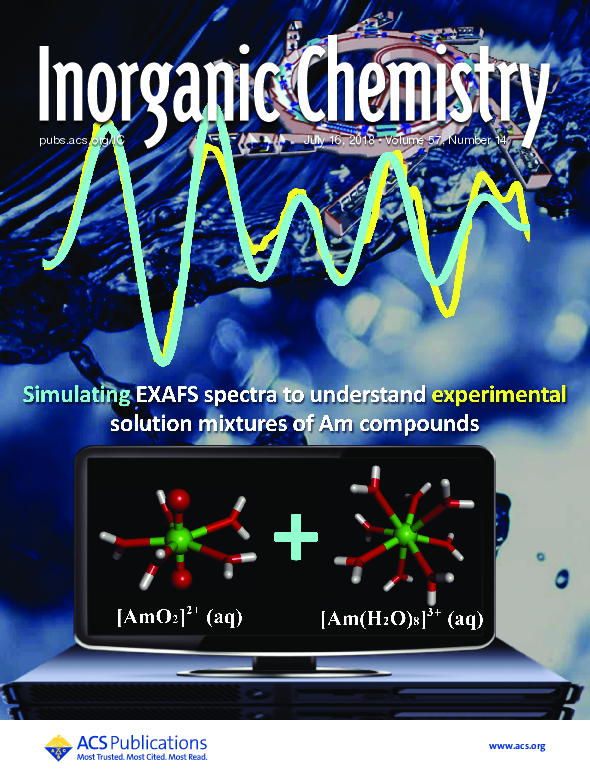
\includegraphics[width=0.5\textwidth]{images/cover_IC2018.png} 
        \caption[Cover Inorganic Chemistry]{Cover of Inorganic Chemistry for the work ``Extracting 
the Americyl Hydration from an Americium Cationic Mixture in Solution: A 
Combined X-ray Absorption Spectroscopy and Molecular Dynamics Study'' presented in this thesis
.\cite{Perez-Conesa2018} }
        \label{cover1}
\end{figure}

Due to its chemical instability, americyl (\ce{[AmO2]^{2+}}), has never been isolated in aqueous 
solution. As a result, the only EXAFS spectrum of \ce{[AmO2]^{2+}} corresponds to a 70/30 mixture 
of 
americyl and \ce{Am^{3+}}.\cite{JRadioanNucChem_Riddle_2016}  We simulated the 
EXAFS spectra of both species from their respective MD simulations and weighted them into a single 
spectrum to produce a simulated EXAFS 
of a mixture of species\cite{Perez-Conesa2018}. The good comparison of the simulated spectrum 
and experiment allowed us to 
predict theoretically the structural parameters and EXAFS spectrum of a pure americyl solution, a 
solution yet to be obtained experimentally\cite{JPC_SPC_2017}. The same procedure was applied 
to the XANES spectrum. This 
work was featured in the cover of the issue 57 of  Inorganic Chemistry of 2018, Figure
\ref{cover1}.



The MD simulations of the uranyl hydrated ion in the aqueous interlayers of 
montmorillonite clays gave interesting microscopical details of the system hard to 
obtain experimentally\cite{JPC_SPC_2017}. The simulations reproduced the few experimental 
microscopical information of 
the system: the uranyl hydrated ion interacts with the surface through the formation of an 
outer-shell complex\cite{GeoCosmoAct_Catalano_2005} and the uranyl axis is neither perpendicular nor 
parallel to the surface\cite{MinWatIntClEq_Denecke_1999}. We 
calculated for the first time from a MD simulation the constrictivity factor, 
$\delta_{int}$, which was found to be near the right order of magnitude to experiment. Strong 
interaction sites for uranyl were found on the clay. These sites are groups of three magnesium 
substitutions around which uranyl cations are electrostatically attracted. As a 
consequence the diffusion of uranyl in the clay exhibits a hopping diffusion mechanism. 
Because of this, the diffusion of uranyl increases with increasing 
uranyl concentration due to cation-cation interactions and a larger coverage of 
surface sites. This work was featured in the cover of the issue 121 of the Journal 
of Physical 
Chemistry C of 2017, Figure \ref{cover2}. In addition it was chosen best article of a young member 
of the ``Specialized Group of atomic and molecular physics'' (GEFAM) of the Royal Spanish 
Society of Physics in 2017.

\begin{figure}[ht!]
     \centering
         
\includegraphics[width=0.5\textwidth]{images/cover_JPCC2017.pdf} 
        \caption[Cover Journal Physical Chemistry C]{Cover of the Journal of Physical Chemistry C 
for the work ``Hydration and Diffusion Mechanism of Uranyl in Montmorillonite Clay: Molecular 
Dynamics Using an Ab Initio Potential'' presented in this thesis.
\cite{JPC_SPC_2017} }
        \label{cover2}
\end{figure}

Finally, a simple local fingerprint for 
hydrophobicity/hydrophilicity was developed. This fingerprint is inspired by the expansion of 
the 
entropy of a system as a sum of terms of increasing correlational 
order.\cite{nettleton1958expression,baranyai1989direct} The fingerprint, which refers to the 
translational component of the entropy, 
measures the hydrophobicity/hydrophilicity of individual atoms of a solute taking as input its 
radial distribution function with water. The fingerprint classifies satisfactorily, the atoms of 
the amino acids. Nevertheless, the fingerprint has mixed results in classifying the atoms of 
the actinyl pentahydrates. A future improved fingerprint should probably make use of orientational 
pair entropy in addition to some techniques to consider the anysotropicity of the solute in 
complex 
environments. Additionally, the fingerprint proved to be a useful solvation/desolvation 
collective variable for enhanced sampling simulations. 

\bibliographystyle{achemso}
\bibliography{./library,./extrabib}